\documentclass[a4paper,12pt]{article}
\usepackage{fullpage}
\usepackage[T1]{fontenc}
\usepackage{amsmath}
\usepackage{amssymb}
\usepackage[utf8]{inputenc}
\usepackage{color}
\usepackage{authblk}
\usepackage{todonotes}
\usepackage{caption}
\usepackage{url}
\usepackage{float}
\usepackage{sectsty}
\usepackage{pdfpages}
\usepackage[section]{placeins}
\DeclareCaptionFont{white}{\color{white}}
\DeclareCaptionFormat{listing}{\colorbox{gray}{\parbox{\textwidth}{#1#2#3}}}
\captionsetup[lstlisting]{format=listing,labelfont=white,textfont=white}

\usepackage{setspace}
\usepackage[toc,page]{appendix}
\usepackage{framed}
\usepackage{geometry}

\usepackage{alltt}
\usepackage{subfig}

% Change section fonts
\allsectionsfont{\sffamily}

% For code box
\usepackage{xcolor}
\usepackage{listings}
\usepackage{caption}
\DeclareCaptionFont{white}{\color{white}}
\DeclareCaptionFormat{listing}{%
  \parbox{\textwidth}{\colorbox{gray}{\parbox{\textwidth}{#1#2#3}}\vskip-4pt}}
  \captionsetup[lstlisting]{format=listing,labelfont=white,textfont=white}
  \lstset{frame=lrb,xleftmargin=\fboxsep,xrightmargin=-\fboxsep}
% End code box

\usepackage{cite}

% General parameters, for ALL pages:
\renewcommand{\topfraction}{0.9}	% max fraction of floats at top
\renewcommand{\bottomfraction}{0.8}	% max fraction of floats at bottom
% Parameters for TEXT pages (not float pages):
\setcounter{topnumber}{2}
\setcounter{bottomnumber}{2}
\setcounter{totalnumber}{4} % 2 may work better
\setcounter{dbltopnumber}{2} % for 2-column pages

\addtolength{\topmargin}{0.5in}

\usepackage{fancyvrb}

\usepackage{tikz} \usetikzlibrary{trees}
\usepackage{hyperref} % should always be the last package

% useful colours (use sparingly!):
\newcommand{\blue}[1]{{\color{blue}#1}}
\newcommand{\green}[1]{{\color{green}#1}}
\newcommand{\red}[1]{{\color{red}#1}}

% useful wrappers for algorithmic/Python notation:
\newcommand{\length}[1]{\text{len}(#1)}
\newcommand{\twodots}{\mathinner{\ldotp\ldotp}} % taken from clrscode3e.sty
\newcommand{\Oh}[1]{\mathcal{O}\left(#1\right)}

% useful (wrappers for) math symbols:
\newcommand{\Cardinality}[1]{\left\lvert#1\right\rvert}
\newcommand{\Ceiling}[1]{\left\lceil#1\right\rceil}
\newcommand{\Floor}[1]{\left\lfloor#1\right\rfloor}
\newcommand{\Iff}{\Leftrightarrow}
\newcommand{\Implies}{\Rightarrow}
\newcommand{\Intersect}{\cap}
\newcommand{\Sequence}[1]{\left[#1\right]}
\newcommand{\Set}[1]{\left\{#1\right\}}
\newcommand{\SetComp}[2]{\Set{#1\SuchThat#2}}
\newcommand{\SuchThat}{\mid}
\newcommand{\Tuple}[1]{\langle#1\rangle}
\newcommand{\Union}{\cup}
\usetikzlibrary{positioning,shapes,shadows,arrows}
\providecommand{\keywords}[1]{\textbf{\textit{Keywords: }} #1}

\title{\textbf{NoSQL: Moving from MapReduce Batch Jobs to Event-Driven Data Collection}}
\author{Lukas Klingsbo}

\begin{document}

%\maketitle
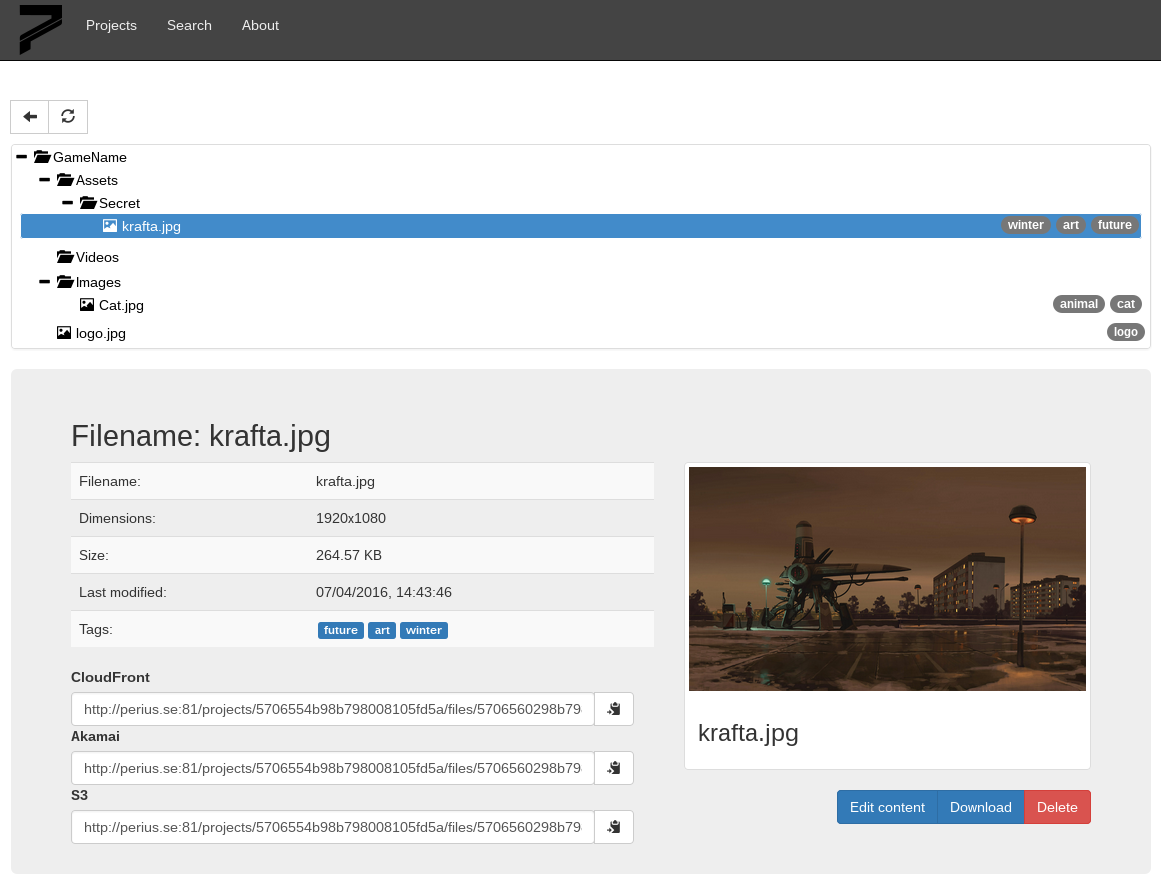
\includepdf[pages={1}]{front.pdf}
\thispagestyle{empty}
\newpage\null\thispagestyle{empty}\newpage

\pagenumbering{roman}
\setcounter{page}{2}

\includepdf[pages={1}]{abstract.pdf}
%\begin{abstract}
%Collecting and analysing data of analytical value is important for many service providers today. 
%Many make use of NoSQL databases for their larger software systems, what is less known is how to 
%effectively analyse and gather business intelligence from the data in these systems. 
%This paper suggests a method of separating the most valuable analytical data from the rest in 
%real time and at the same time providing an effective traditional database for the analyser. 
%
%In this paper we analyse our given data sets to decide whether big data tools are required and 
%then traditional databases are compared to see how well they fit the context. 
%A technique that makes use of an asynchronous logging system is used to insert the data from the 
%main system to the dedicated analytical database. 
%
%The tests show that our technique can efficiently be used with a traditional database even on large 
%data sets (>1000000 insertions/hour per database node) and still provide both historical data 
%and aggregate functions for the analyser.\\
%
%\keywords{NoSQL, data mining, data collection, DBMS benchmark, business intelligence, analytical logging}
%\end{abstract}

\newpage\null\thispagestyle{empty}\newpage

\setcounter{tocdepth}{3}
\tableofcontents

\clearpage
\pagenumbering{arabic}
\setcounter{page}{1}
\section{Introduction to the\\"Big Data/NoSQL problem"}
In times when big data collection is growing rapidly~\cite{E1} companies and researchers alike face the problem of doing analysis of the data that has been collected.
The enormous amounts of data collected are often saved in distributed big data databases or key-value stores with fast insertion operations but with comparatively slow and complex (but highly parallelizable) query functions~\cite{RT1}.
This work tries to solve such a problem at Kivra~\cite{KIVRA}, a company working to digitalise and minimise the use and need of conventional paper mail. To gather analytical data from Kivra's distributed database today requires heavy Map/Reduce 
queries. To do day to day analysis of the data slowly becomes unbearable and non-scalable as it takes several hours or even days to run a Map/Reduced~\cite{G1} batch job to fetch the data that is going to be analysed.
The solution proposed and examined by this paper is to structure and asynchronously collect data after interesting events occur, that are of a high analytical value, into a smaller and more easily queryable database.

\newpage
\section{Related Terminology}

\subsection{Big data}
Big data~\cite{BD1} is a loose term for ways of collecting and storing unstructured complex data of such large volumes that normal methods of data manipulation and querying can not be used.

\subsection{NoSQL}
NoSQL~\cite{NOSQL} is a term that have not fully settled its meaning, it started by meaning no relational databases~\cite{NOSQL}, but now it has moved on to commonly be referred to as Not Only SQL. 
If a database calls itself NoSQL it usually means that is is non-relational, distributed, horizontally scalable, schema-free, eventually consistent and support large amounts of data~\cite{NOSQL2}.

\subsection{MapReduce}
MapReduce~\cite{G1} is referring to a programming model that makes parallel processing of large data sets possible. In simplified terms it consists of two functions, one called Map and one called Reduce.
The Map function is sent out to each node from a master node and the function is separately executed on each nodes data set and then each node assembles the result back together with the other nodes so that all 
input values with the same results are grouped together. Then the reduce function is executed, either in parallel or on a master node, and this function does calculations upon each separate result list with the data from all nodes that 
ran the Map function and it then combines the input from them to the answer that was originally inquired.

\subsection{Eventual consistency}
The expression eventual consistency is a term used for describing how data is processed in database systems. Eventual consistency means that the data may not be consistent in any one moment, 
but will eventually converge to being consistent~\cite{EVENTUAL}. This makes it possible for distributed databases to operate faster as data does not have to be locked during insertions, updates 
and deletion and thus does not have to be propagated to all nodes before more actions on the same data can be sent to a node. If one or more nodes operate on the same data as another node 
whose changes have not propagated through the system yet, the system will have to handle in which order the operations should be performed, this is usually called sibling or conflict resolution~\cite{RESOLUTION}.

\subsection{Riak}
Riak is a key-value datastore that implements NoSQL concepts such as eventual consistency. It is usually configured to run with at least 5 nodes to be as efficient as possible.
To query the datastore you either use the REST-ful API or MapReduce functionality that it provides.

Riak~\cite{RIAK} provides fault tolerance and high availability by replicating data to several nodes, the default is to have all data replicated to three nodes.

\subsection{Lager}
Basho~\cite{BASHO}, the company that developed Riak~\cite{RIAK}, has developed a modular logging framework called Lager~\cite{LAGER}. Lager is modular in the sense that it is possible to write separate backends 
which all can separately do asynchronous data collection. As the system performance can not be noticeably affected by adding a subsystem to collect analytically valued events it is of highest priority 
that they can be sent asynchronously so that the implication of implementing such a subsystem wont result in delays for the main system. 

A problem that these form of logging systems can experience is that the events that they have to handle queue up faster than they can be processed. To solve this Lager~\cite{LAGER} has a built-in overload protection 
to make sure that its message queue will not overflow. It does this by swapping synchronous and asynchronous messaging for the separate backend.

\subsection{Abbreviations}

\subsubsection{RDBMS}
RDBMS~\cite{RDBMS} is an abbreviation for relational database management system. This is the most commonly used database management system and is usually referred to as a traditional database. Data is stored within tables and data can be in relation to each 
other across tables and such databases are therefore called relational.

\subsubsection{DDBMS}
DDBMS~\cite{DDBMS} is an abbreviation for distributed database management system. It is used to centrally manage a distributed database system and to give the user the impression and functionality as though the database system 
would run on only one node.

\newpage
\section{Background}
\subsection{About Kivra}
Kivra~\cite{KIVRA} is a company which aims to digitalise and eliminate the use of superfluous analogue paper mail. 
They do this by making it possible for companies and governments to send documents digitally to customers or citizens. 
By tying the users' accounts to their social security numbers in the service the sender can be sure that the document 
reaches the correct recipient. 

Today Kivra has a continuously growing user base of more than 500.000 users, according to their website~\cite{KIVRA}. 

\begin{figure}[h!]
    \vspace{0.25in}
    \centerline{\includegraphics[scale=0.4]{kivraui}}
    \caption{The user interface of Kivra}
    \label{fig:ui}
\end{figure}

As can be seen in figure~\ref{fig:ui}, the interface reminds of the interface of any email provider, however the documents sent to the users can be interactive and have a more advanced layout and the main advantage over normal email is that every 
users identity is established in the registration process. 
The user can validate its identity either by using mobile BankID~\cite{BANKID} or by receiving an activation code to its registered place of residence. 
This advantage makes it possible for companies and organizations that otherwise would have had to send documents to a registered postal address to being able to send them digitally through Kivra. 


\subsection{The current system}
Kivra's users interact with the backend system (this is the backend box represented in Figure~\ref{fig:before}) either through Kivra's web page or their app, where they can receive documents, pay bills, set whom they accept documents from and also set personal details. 
Users sign up either though mobile bankID or requests an activation code to be sent to the address registered to their social security number, this is to ensure the identity of the user. 
When a user receives a new document it is notified through email or SMS and can then log in to read the document. 

The data which is of analytical interest is information about the users, meta data of the documents sent out to the users and whether a user accepts or does not accept (internally called \emph{send requests}) documents from a company or organization (internally called a \emph{tenants}).

\newpage
\subsection{Problem description}
The part of the current system that is being examined consists of Riak, a distributed key-value datastore, and a batch script containing MapReduce queries which are running each night to collect 
data to a PostgreSQL database which is later used for deeper analysis. This system architecture can be seen in Figure~\ref{fig:before}. 
The batch script is emptying all of the analytically interesting buckets in the Riak cluster,
currently there are two buckets being emptied every night. One of them contains send requests which is meta data telling the system if a user accepts documents for a specific tenant and the other bucket
just contains plain user information. In the future meta data regarding documents sent to users will be collected as well.

This solution does not scale and is also inefficient as you have to go through all the data in the growing buckets that are of interest every night, instead of accumulating the data to a separate database dedicated for analysis 
at the same time as you insert or change data in Riak.

\begin{figure}[h!]
    \vspace{0.25in}
    \centerline{\includegraphics[scale=0.7]{system_before}}
    \caption{The analytical system at Kivra}
    \label{fig:before}
\end{figure}

~\\
\newpage
\section{Methods for determining\\implementation details}
This chapter introduces the different methods used to determine how the new system should be implemented, which DBMS it should use and how the estimation of long term scaling was done.

\subsection{Data size and growth estimation}
The data size and growth was estimated with statistics collected from the current Riak cluster in Kivra's system. What the current insertion rate would be like with an event driven implementation was estimated 
by doing SQL queries measuring the number of insertions that could be made within certain time limits. 
To estimate the size and growth of the future database implementation both past estimations and the current internal estimated growth of the company were used. 
This, together with the scalability measurements, was required to make sure that the solution would be durable in the long run.

\subsection{Scalability measurement}
The scalability was estimated for the typical server hardware of Kivra with the different databases and with statistics of growth estimations from the current database. 
This was necessary to make sure that the system would scale with the expected data growth, within a reasonable time frame. 

\subsection{DBMS comparison}
The database management systems were compared by testing required abilities and examining load and speed by running insertion jobs of different sizes. 
The DBMSs architecture and suitability were also compared to see which one suited the context best. 
These comparisons were vital to make sure that the chosen DBMS could handle the expected load of the system. 

\newpage
\section{Solution for storing events}
When an event of analytical interest occurs, an asynchronous call with information about the event is sent to Lager. Lager then directs it to an in-house tailored Lager backend, which is responsible for 
making sure that the data is stored consistently and correctly. The database in which the data is stored can then be queried at any time to perform near to real time analysis of the system. 
After analysing internal database statistics an approach of this form is estimated to cause approximately 100-10000 inserts/hour depending on if it is during the peak hours or not. The estimation can not be averaged as 
the chosen database is required to be able to handle the peak hours without a problem. This approach will lead to a system with no updates and only reads during analytical calculations. This is due to the fact that 
the backend will handle each event with a strict progression of inserting the relevant metadata of the event with a timestamp and never have a need of updating, nor removing old data, as all of these 
chosen events are valuable to store to enable historical queries. This is similar to how Lager~\cite{LAGER} logs events to files, except that the analysis of the data will be easier due to the 
built-in aggregate functions of modern databases. In comparison to the current system it will be possible to perform near to instant analysis of the data already collected instead of having to re-collect all 
the data of analytical interest from the Riak cluster each time an up-to-date analysis of the data has to be performed.

\subsection{Data sets}
\subsubsection{Determining the type of the data sets}
Big data is one of the popular buzzwords in the computer industry today and a lot of revolutionising technology has been built around it. But it is not always efficient to use technology built for 
these data sets if the data set that is being operated on does not fit the definition of big data. But as there is a thriving hype of higher yield with existing data some companies and institutions use it 
just for the sake of being part of the trend without actually having a data set that objectively would be classified as big data~\cite{NOTBIG}.


To simplify the abstract definition of Big Data to determine whether a data set can be defined as such you can classify the data set by concluding the answers of 
three questions~\cite{BD1}, namely the following:
\begin{itemize}
    \item Is the data set large?
    \item Is the data set complex (maybe even unstructured)?
    \item Are methods optimized for other data sets inefficient?
\end{itemize}

If the data set satisfies these properties it can be a good idea to store the data in a Hadoop cluster or similar technology developed specifically for big data. 
If, however, the data set does not satisfy these criteria it is usually better to look for another storage solution~\cite{NOTBIG}.

At Kivra there are a few different data sets with information that is valuable for ongoing analysis. 
The three most important data sets are: 
\begin{itemize}
    \item User information - each users personal details.
    \item Send requests - connects a user to a tenant and specifies whether the user wants or does not want content from that specific tenant.
    \item Content metadata - contains meta data of content that has been sent to users. 
\end{itemize}
~\\
The tables representing this data would be quite simple and would not store too much information as analysis of the system would mostly regard metadata of some of the information stored in the Riak cluster.
See an example of how such tables could look like in listing~\ref{example_tables}.

\begin{lstlisting}[label=example_tables,caption=Example tables]
Example fields of the tables
+-------------+  +--------------+  +------------------+
| User        |  | Send request |  | Content Metadata |
+-------------+  +--------------+  +------------------+
| id          |  | user_id      |  | content_id       |
| name        |  | tenant_id    |  | tenant_id        |
| address     |  | accepted     |  | user_id          |
| city        |  | timestamp    |  | timestamp        |
| email       |  |              |  |                  |
| timestamp   |  |              |  |                  |
+-------------+  +--------------+  +------------------+
\end{lstlisting}

\subsubsection{Size of the data sets}
\label{DATASETSIZE}
As each record in the data sets is fairly small (under 200 bytes) it is enough to count the number of records plus the expected growth for the future. Today there are about 500 000 users with information~\cite{KIVRA}. 
The send requests records adds up to a little bit less than the number of users times the number of tenants and then there is also around 2 million content records. This results in a total of about 10 million records. 
All of the data sets have an expected growth of about 5\% per month according to internal statistics of Kivra collected from their Riak cluster. This is well within the limits of traditional relational databases~\cite{SQLPERF}.

\subsubsection{Complexity of the data sets}
None of the data sets have any complex structures, the data types are not varying and there are no big documents that requires to be stored in the analytical database as only the meta data of the content being 
sent to users has to be saved and not any attachments, images etc.

\subsubsection{Inefficiency of other methods}
There is no need for extremely fast reads for specific values which key-value stores~\cite{KEYVALUESTORE} offer or for extremely fast insertion rates which big data databases~\cite{BD1} can provide. 
As concluded in the section about the size of the data sets (~\ref{DATASETSIZE}) and the section called Choosing SQL database (~\ref{SQLDATABASES}) the insertion rate of 
traditional databases will be well above the demands. As there is no complex data the normal table structure of a RDBMS will be suitable for storage of the data. 

\newpage
\subsection{Protocols for data transfer}
The requirements of the protocol and data structure used to transfer and translate data to the database differs highly on what type of data and from where the data is being sent, some data are required to have 
absolute transport security and reliability meanwhile other is of lower importance and rather trades transport reliability for speed. To maximize the speed and flexibility of the system as a whole, 
one or several APIs and web services that can accept several protocols and differently structured data being used towards it before translating it in order to store it in the database should be used, as can be seen in 
Figure~\ref{fig:api}.

The exact APIs, Web Services and data structures used for the implementation of this system is outside the scope for this work and will be left to a future implementer to decide. But examples of such protocols 
could be HTTP through a RESTful~\cite{REST} service, cURL~\cite{CURL} with one of its many supported protocols or simply whatever protocol that will be built in to the customised Lager~\cite{LAGER} backend.

\begin{figure}[h!]
    \vspace{0.25in}
    \centerline{\includegraphics[scale=0.7]{system_api}}
    \caption{API explanation}
    \label{fig:api}
\end{figure}

\subsection{Database}
\subsubsection{Requirements}
\label{REQUIREMENTS}
As the database will mostly be used for insertions, the insert operations will have to be as fast as possible with the chosen way to store the data. 
Read operations will not have to be very fast as they are not directly used by any response time critical system but rather by in-house users, a business intelligence system or a system providing an interface of generated 
graphs and tables for overviewing the information. 

The requirements on the speed of updates and deletes are non essential as they will only occur when manually editing the database. 
The database will not have to be portable, it is not going to be replicated or moved around. 
For future scaling of the database it is needed to be easily configurable and preferably have wide support for distribution of the data over several nodes. 
The data is required to be accessible and easy to aggregate upon for future analysis.

\subsubsection{Why SQL over NoSQL?}
A traditional relational database system was chosen over a NoSQL document store or key-value store for a few different reasons.
The first reason was that the high insertion rate trade off that results in eventual consistency~\cite{EVENTUALCONS} given by NoSQL databases would simply not be needed as the amount of data insertions and updates would 
be well within the limits of a traditional RDBMS~\cite{SQLPERF} as can be seen in Section~\ref{SCALABILITYRESULT}.

The second reason was that the query speed of specific values, offered by key-value stores~\cite{KEYVALUESTORE}, was not required and the demand was rather for a full set of aggregate 
functions and easy access to complete subsets of the stored data. 
As many NoSQL databases use MapReduce for fetching data it would per definition be hard to write efficient joins and no built in aggregate functions would be provided~\cite{COMP}. 

What was also considered was putting a layer on top of a regular NoSQL database that seamlessly provided this type of functionality. 
The layers considered were HIVE~\cite{HIVE}, PIG~\cite{PIG} and Scalding~\cite{SCALDING} for HADOOP~\cite{HADOOP}. But as the implementation did not need the special functionalities and speed trade-offs, 
which is deeper explained in Section~\ref{SCALABILITYRESULT} and Section~\ref{REQUIREMENTS}, that were offered by such layers the conclusion was to simply incorporate a traditional SQL database. 

\subsubsection{Choosing SQL database}
\label{SQLDATABASES}
There are a large number of different traditional database systems being actively developed today. For this project the focus has been on popular open source DBMSs. 
The most popular open source relational database management systems~\cite{POPULARDBMS} today are MySQL, PostgreSQL and SQLite so the tests compare those towards each other and the requirements. 

\newpage
\paragraph{MySQL}
~\\
MySQL\cite{MYSQL} is the most popular open source database and has several popular forks as well, with the biggest one~\cite{POPULARDBMS} called MariaDB~\cite{MARIADB}. MySQL does not aim at implementing 
the full SQL standard, but rather a subset of it with some extra features~\cite{POPULARDBMS}. MySQL is built in layers with one or several storage engines in the bottom and an optimizer, parser, 
query cache and connection handling layers built on top of that~\cite{HIMYSQL}, see Figure~\ref{fig:mysql}.

\begin{figure}[h!]
    \vspace{0.25in}
    \centerline{\includegraphics[scale=0.7]{mysql}}
    \caption{MySQL Architecture~\cite{HIMYSQL}}
    \label{fig:mysql}
\end{figure}
~\\

MySQL has a rich set of aggregate functions which are very useful when doing statistical analysis of the stored data. In total, MySQL has 17 aggregate functions in which the most common SQL standard 
aggregate functions AVG, COUNT, MAX, MIN, STD and SUM are included~\cite{MYSQLAGG}.

\FloatBarrier
\newpage
\paragraph{PostgreSQL}
~\\
PostgreSQL is one of the few modern SQL databases that implements the whole SQL standard (ANSI-SQL:2008) ~\cite{POSTGRESSTANDARD}. 
The architecture of PostgreSQL is quite straight forward, as can be seen in Figure~\ref{fig:postgres}. The postmaster handles new connections and spawns a PostgreSQL backend process that the client can directly communicate with. All communication 
between client and PostgreSQL goes through that process after it spawns. The postmaster stays active and awaits new incoming connections. Each backend that a client is connected to has its own separate 
parser, rewrite system, optimiser and executor. All of the active backends then uses the same storage engine~\cite{POSTGRES}. PostgreSQL, compared to MySQL, only has one very tightly integrated 
storage engine that in theory could be replaced but that has not been done in practice yet~\cite{POSTGRESQLPAPER}.

\begin{figure}[h!]
    \vspace{0.25in}
    \centerline{\includegraphics[scale=0.7]{postgres}}
    \caption{PostgreSQL Architecture~\cite{POSTGRES}}
    \label{fig:postgres}
\end{figure}
~\\

PostgreSQL have a comparatively large set of aggregate functions including 14 general purpose functions and 18 functions mainly used for statistics, totalling in 32 functions~\cite{POSTGRESAGG}.

\newgeometry{top=2.0cm}
\paragraph{SQLite}
~\\
SQLite as opposed to MySQL and PostgreSQL is not built as a traditional two tier architecture which can be seen in Figure~\ref{fig:sqlite}.
This leads to that each call to it is done through function calls to a linked SQLite library~\cite{SQLITEDEV}. SQLite is quite small (658KiB) and has therefore become widely used as an embedded database 
for local storage~\cite{SQLITE}. SQLite is bundled with two storage engines, one of them is built with a log-structured merge-tree and optimised for persistent 
databases and the other one is built on a binary tree which is kept in memory which makes it suitable for temporary databases. The architecture of SQLite has made it possible to design and interchange 
new storage engines with the built-in ones~\cite{SQLITEENGINE}.

\begin{figure}[h!]
    \vspace{0.25in}
    \centerline{\includegraphics[scale=0.7]{sqlite}}
    \caption{SQLite Architecture~\cite{SQLITE}}
    \label{fig:sqlite}
\end{figure}
~\\

SQLite has 9 of the most basic aggregate functions and lacks the more statistical functionality such as for example standard deviation and covariance that PostgreSQL and MySQL implement~\cite{SQLITEAGG}. 
SQLite's architecture is very focused on portability~\cite{SQLITE} and have made some trade-offs in order to achieve that, as can be seen in its simplistic architecture in Figure~\ref{fig:sqlite}. 
One result of these trade-offs is that insertions become very slow, $\sim60$ insertions per minute with transactions enabled~\cite{SQLITESLOW}.

As portability is not required for the implementation of the system regarded in this paper, because it is missing many important aggregate functions and because of its slow insertion rate, 
SQLite will be excluded from the tests in the next section. 

\newpage
\subsubsection{Performance tests}
As explained in section~\ref{SQLDATABASES}, SQLite was excluded from the tests as its architecture was deemed unfitting for the task at hand and for the lack of many aggregate functions.
The statistics were generated on an average consumer computer with the following specifications:

\vspace{0.25in}
\textbf{CPU:} Intel Core2 Duo T7700 2.40GHz 

\textbf{RAM:} SODIMM DDR2 Synchronous 667 MHz 2x2GB

\textbf{Disk:} KINGSTON SV300S3 120GB SSD partitioned with EXT4

\textbf{OS:} Debian Jessie (Testing)

~\\
PostgreSQL version 9.4 and MySQL version 5.6 were used during the tests and the packages were installed from the default Debian testing repositories.

~\\
The database and table were created in the same manner on both systems as can be seen in listing~\ref{database_creation}.
\begin{lstlisting}[label=database_creation,caption=Database and table creation]
create database testdb
create table test_table 
    (data varchar(100), 
    moddate timestamp default current_timestamp);
\end{lstlisting}

The tests were conducted with a series of simple insertions containing random data, as shown in listing~\ref{test_table}.
\begin{lstlisting}[label=test_table,caption=Example insertion]
insert into test_table (data) 
values ('010100100101010100...');
\end{lstlisting}

The execution times were measured by using the time~\cite{TIME} utility of the GNU project, it measures the time of execution and resource usage of the specified operation. 
The different files that were used in the tests contained 1000, 10 000, 100 000 and \\1 000 000 insertions of random data. 
When deploying this system the production servers will most likely be a lot more powerful than the consumer laptop that these test were run on.
These tests non the less gives a correct representation of how well the different databases will scale. 
To reproduce or verify the results, see listings 3 and 4 in Appendix~\ref{appendix:a}.

\begin{figure}[h!]
    \vspace{0.25in}
    \centerline{\includegraphics[scale=0.7]{linegraph2}}
    \caption{Performance graph}
    \label{fig:vs}
\end{figure}

As can be seen in Figure~\ref{fig:vs} both of the systems have a very close to linear performance and any small disturbances in the pattern can be concluded to be from other processes using system resources.
Both of the systems perform over the preconditions for an implementation with requirements similar to the ones in this context. But as insertion rate and aggregate functions are of high concern for such 
an implementation and both systems comply to the rest of the requirements, PostgreSQL will be recommended to use for a future implementation.

\newpage
\subsection{Storage requirements}
As the data comes in as events, there is never a need to update old records in the database, as can be seen in Figure~\ref{fig:storage}. This structure is slightly harder to do complicated 
queries (Listing~\ref{fetch_example}) towards, as you always have to take the timestamp of the event into consideration. 
But it also makes it possible to configure the DBMS not to lock tables during inserts, which will increase the speed of insertion of the database. The lack of locks will be especially useful if it is later 
decided to use a DDBMS for an eventual requirement of scaling up the system in the future. As everything is logged with timestamps it is particularly suitable for business intelligence systems and the likes of such, as you can query 
time ranges in the past as well as the current state of the system to gather analytics and make comparisons. 

\begin{figure}[h!]
    \vspace{0.25in}
    \centerline{\includegraphics[scale=0.6]{system_dbms}}
    \caption{Flow of data}
    \label{fig:storage}
\end{figure}

The only time inserts occur is during the time when the customised Lager~\cite{LAGER} backend or later added data sources sends events (1, see Figure~\ref{fig:storage}) and the only times reads are performed 
is when a manual query (2, see Figure~\ref{fig:storage}) is executed or when an eventual business intelligence system or an automated analyse system (3, see Figure~\ref{fig:storage}) that automatically queries the system is used. 
It will never be necessary to perform updates and no regular deletes will have to be performed, as explained in Section~\ref{REQUIREMENTS}.

The actual database size should not be a problem as the servers are usually equipped with a few terabytes of disk space. An average insertion of Kivra is estimated to around 200 bytes by looking at meta data formed by data currently in the Riak cluster.
This means that $5*10{^9}$ insertions would fit on a disk with 1TB of space. A rough estimation of an average of 5000 insertions per hour means that a 1TB would last for more than 113 years, see Figure~\ref{fig:storage2}.

\begin{figure}[h!]
\begin{framed}
\begin{enumerate}
\item $1TB/200B \thickapprox 5*10^{9}$ insertions
\item $5*10^{9}/5000/24/365 \thickapprox $ 113.5 years
\end{enumerate}
\end{framed}
\caption{Estimation of disk space usage}
\label{fig:storage2}
\end{figure}

\FloatBarrier
\newgeometry{top=2.0cm}
\newpage
\section{Resulting system}
The result of an implementation of the suggested solution of this paper would lead to a core system that would have a data flow as described in Figure~\ref{fig:result}.
In this flow, when data of analytical interest would be inserted into the Riak cluster it would also be sent to Lager which would insert it into a RDBMS dedicated for 
analytical data, instead of fetching data in Riak after it has been inserted as was it done in the previous systems data flow that can be seen in Figure~\ref{fig:before} and explained in Section 3.2.

\begin{figure}[h!]
    \vspace{0.25in}
    \centerline{\includegraphics[scale=0.7]{system_after}}
    \caption{Resulting system}
    \label{fig:result}
\end{figure}

What is not shown in Figure~\ref{fig:result}, is that separate data sources for the analytical database can be used. These can connect with different protocols and with differently 
structured data to an API that will be receiving data for the database as described in Section 5.2.

\subsection{Scalability}
\label{SCALABILITYRESULT}
If an unoptimised PostgreSQL database on an average consumer computer is used and with the assumption that little to no data transfer latency will occur during insertion of data the insertion rate can 
be increased by a factor of at least 100 if following the upper boundary of the estimation (Section 5) of 10000 insertions per hour. As can be seen in the load test in 5.3.4, PostgreSQL can handle a little bit over 
1 million insertions per hour. The expected data growth rate is 5\% per month, with this growth the same setup could be used for almost 8 years, see Figure~\ref{fig:scalability}.

\begin{figure}[h!]
\begin{framed}
\begin{enumerate}
\item $10000*1.05^{94} \thickapprox $ 981282 insertions/hour 
\item $94/12 \thickapprox $ 7.83 years 
\end{enumerate}
\end{framed}
\caption{Estimation of data transfer scaling}
\label{fig:scalability}
\end{figure}

In the unlikelihood that the same setup with the same hardware and PostgreSQL version would be used in 8 years the PostgreSQL database could easily be sharded, clustered or optimised to reach a lot higher 
insertion rates. As all he data is independent and has no defined relations to other data, clustering with a pool of independent databases could be used without any requirement of the databases to synchronise with each 
other, this would mean that you can linearly add 1000000 insertions/hour for each database node that you add to the cluster.

\subsection{Practical Example}
\subsubsection{Storing an Event}
After an implementation of a solution like this at Kivra the following would be the flow of a typical change triggered by a user. 
The system would update the send request bucket of Riak in Figure~\ref{fig:practical}, but changes to other buckets would look exactly the same. 

Figure~\ref{fig:practical} is a practical example of what would happen if a user updated his or her preferences of which tenants it wishes to receive documents from.

\begin{figure}[h!]
    \vspace{0.25in}
    \centerline{\includegraphics[scale=0.7]{practical_flow}}
    \caption{Practical example of a send request changing}
    \label{fig:practical}
\end{figure}

\newpage
\subsubsection{Querying Data}
To query data stored in the analytical database a query that takes the timestamps into consideration has to be performed. The query in listing~\ref{fetch_example} is an example of how to query which 
tenants all users wish and do not wish to receive documents from. Queries for other data sets would look similar.

\begin{lstlisting}[label=fetch_example,caption=Example query]
SELECT SRQ.user_id, SRQ.tenant_id, SRQ.timestamp, SRQ.accepted 
FROM sendrequest SRQ 
INNER JOIN 
  (SELECT user_id, tenant_id, max(timestamp) as latest
   FROM sendrequest GROUP BY user_id, tenant_id) SRQ1 
ON SRQ.user_id = SRQ1.user_id 
AND SRQ.tenant_id = SRQ1.tenant_id 
AND SRQ.timestamp = SRQ1.latest;
\end{lstlisting}

The query in listing~\ref{fetch_example} doesn't take into consideration if the same name and tenant combination exists with the same timestamp. 
It is however highly unlikely that it would happen as the timestamps are stored with a micro second precision. 
To fully avoid that event, add an auto incremented ID column to the table and only consider the highest ID in the case of a clash.

\newpage
\section{Discussion}
\subsection{Event-driven data collection}
The suggested solution introduced by this paper was named event-driven data collection. The name has been used before for slightly similar purposes with the first recorded case 
being in 1974~\cite{EVENTDRIVEN}. It has also been used in a different manner in quite a few papers on the subject wireless sensor networks~\cite{EVENTDRIVEN2} and some regarding the collection of natural 
ionosphere scintillations~\cite{EVENTDRIVEN3}.

\subsection{Flat file database}
A flat file database was not compared in this paper because of the precondition of having pre-built APIs and to give easier access to querying and aggregation of data. A flat file database can also be complicated to scale out 
to several servers for an eventual future requirement. 

\newpage
\newgeometry{top=4.0cm}
\section{Summary}
\subsection{Conclusions}
The system that has been designed in this paper can be used as an effective tool for logging and analysing events. This form of approach is especially valuable if the main system is using some form of MapReduce 
database which can be hard to do ongoing analysis of aggregated data on. If the main system is already using a SQL database as its primary form of information storage this type of solution would be quite inefficient 
due to duplication of data and possibly having to serve another DBMS\@. In the benchmarking of the different database management systems the standard version without modifications have been used, with modifications 
and optimisations the outcome would have been very different. 

The unorthodox design of the database schema in this paper provides a full historical log of events which makes it possible to compare data from different time ranges, 
which can be very valuable when analysing data from business systems to for example detect trends and tendencies within the user base. 

Another contribution of this work is the use of a logging system to effectively put in an analytical systems 
to an already existing backend with minimal impact on the performance of the existing system. 

\subsection{Future work}
To finalise the architecture of this system, APIs and web service structures will have to be researched or developed to be put on top of the database. For larger flows of data other solutions would have 
to be considered or alternatively the used DBMS has to be heavily optimised by for example removing insertion locks. Scaling out to a clustered database could also be an alternative.

\newpage
\newgeometry{top=2.0cm}
\begin{appendices}
\section{Benchmarks}
\label{appendix:a}
\begin{lstlisting}[label=some-code,caption=PostgreSQL insertion test]
1 000 000 insertions
$ time psql --quiet -f test4.sql
psql --quiet -f test4.sql
40.42s user 23.08s system 2% cpu 31:05.03 total

100 000 insertions
$ time psql --quiet -f test.sql
psql --quiet -f test.sql
4.32s user 2.38s system 2% cpu 5:02.94 total

10 000 insertions
$ time psql --quiet -f test2.sql
psql --quiet -f test2.sql
0.51s user 0.22s system 2% cpu 30.172 total

1000 insertions
$ time psql --quiet -f test3.sql
psql --quiet -f test3.sql 
0.11s user 0.02s system 4% cpu 3.077 total
\end{lstlisting}
\begin{lstlisting}[label=some-code,caption=MySQL insertion test]
1 000 000 insertions
$ time mysql -u root -p********** testdb < test4.sql
mysql -u root -p********** testdb <   
39.78s user 23.36s system 1% cpu 1:36:56.31 total

100 000 insertions
$ time mysql -u root -p********** testdb < test.sql
mysql -u root -p********** testdb < 
3.88s user 2.83s system 1% cpu 9:22.67 total

10 000 insertions
$ time mysql -u root -p********** testdb < test2.sql 
mysql -u root -p********** testdb < 
0.31s user 0.39s system 1% cpu 53.174 total

1000 insertions
$ time mysql -u root -p********** testdb < test3.sql 
mysql -u root -p********** testdb < 
0.08s user 0.00s system 1% cpu 5.318 total
\end{lstlisting}
\end{appendices}
\restoregeometry


\newpage
\bibliographystyle{ieeetr}
\bibliography{references}

\end{document}
